\documentclass[addpoints]{exam}

% \pagestyle{empty}                       %no page numbers
% \thispagestyle{empty}                   %removes first page number
% \setlength{\parindent}{0in}               %no paragraph indents

\usepackage{fullpage}
\usepackage[tmargin = 0.5in, bmargin = 1in, hmargin = 1in]{geometry}     %1-inch margins
\geometry{letterpaper}                  
\usepackage{graphicx}
\usepackage{amssymb}

% Default packages
\usepackage{latexsym}
\usepackage{amsfonts}
\usepackage{amsmath}
\usepackage{amsthm}
\usepackage{hyperref}
\usepackage{multicol}
\usepackage{multirow}
\usepackage{enumerate}
\usepackage{enumitem}

\def\pageturn{\vfill
\begin{flushright}
	\begin{small}
		Continued $\rightarrow$
	\end{small}
\end{flushright}
\newpage}

\pagestyle{headandfoot}
\runningheadrule
\firstpageheader{\textbf{MTH 201-07 (Talbert)}}{\textbf{Final Exam --- \numpoints \ points}}{\textbf{December 11, 2013}}
\runningheader{MTH 201}
{MTH 201-07 Final Exam, Page \thepage\ of \numpages}
{Dec 11, 2013}
\firstpagefooter{}{}{}
\runningfooter{}{}{}

\begin{document}

		
\vspace*{0pt}

\noindent
Name: \underline{\hspace{2in}} \\


\noindent
\textbf{Instructions}:  You may use an $8.5 \times 11$ inch sheet of paper with notes on it as well as a calculator. Except on multiple choice questions, you need to show all work in a clear and complete way to receive credit. 

\begin{questions}

\uplevel{\emph{Items 1---10 are multiple choice questions that address a variety of learning objectives. Please circle the ONE response you believe is most correct. You do not need to justify your answer.}}

\question[2] The derivative $f'(a)$ of a function $f$ at the point $x=a$ tells us
	\begin{parts}
		\part The average rate of change of $f$ at $x = a$
		\part The slope of the tangent line to $f$ at $x=a$
		\part The height of the graph of $f$ at $x = a$
		\part All of the above
		\part Just (a) and (b)
	\end{parts}
	

% \question[2] The tangent line to the graph of a function $g$ at the point $(2, 4)$ goes through the point $(5, -11)$. The value of $g'(2)$ 
% 	\begin{parts}
% 		\part Equals $-11$ 
% 		\part Equals $-5$ 
% 		\part Equals $4$
% 		\part Equals $5$ 
% 		\part Cannot be determined from this information alone
% 	\end{parts}
	
\question[2] The graph of a function $T$ passes through the points $(1,2)$ and $(3, 8)$. From this information alone, we can conclude
	\begin{parts}
		\part The average rate of change in $T$ on $[1,3]$ is positive 
		\part $T'(1)$ is positive 
		\part $\int_1^3 T(x) \, dx$ is positive 
		\part All of the above
		\part Just (a) and (b) 
	\end{parts}

\question[2] If $f$ is an antiderivative of $g$ and $g$ is an antiderivative of $h$, then 
	\begin{parts}
		\part $h$ is an antiderivative of $f$
		\part $h$ is the derivative of $f$ 
		\part $h$ is the second derivative of $f$
		\part $h$ is the derivative of $f''$
		\part None of the above
	\end{parts}


	% \question[2] Which of the following is a correct definition of the derivative of a function $f(x)$? 
	% \begin{parts}
	% 	\part $\displaystyle{\lim_{h \to 0} \frac{f(x+h) - f(x)}{h}}$
	% 	\part $\displaystyle{\lim_{x \to 0} \frac{f(x+h) - f(x)}{h}}$
	% 	\part $\displaystyle{\lim_{h \to x} \frac{f(x+h) - f(x)}{h}}$
	% 	\part $\displaystyle{\lim_{x \to h} \frac{f(x+h) - f(x)}{h}}$
	% 	\part $\displaystyle{\lim_{h \to 0} \frac{f(h) - f(x)}{h}}$
	% \end{parts}	


\question[2] A function $y = g(x)$ is such that $g'(2) = -3$. From this information alone, we can conclude that 
			\begin{parts}
				\part The graph of $g$ is below the $x$-axis at $x = 2$
				\part The graph of $g$ is decreasing at $x = 2$
				\part The graph of $g$ is concave down at $x = 2$
				\part Just (a) and (b)
				\part None of the above
			\end{parts}
	
\question[2] For any function $y = g(x)$, if $g''(x) > 0$, it means that 
	\begin{parts}
		\part $g$ is positive 
		\part $g$ is increasing
		\part $g$ is linear with a positive slope
		\part $g$ is concave up
		\part No conclusions can be drawn about $g$ based on this information
	\end{parts}
	
	\pageturn
	
	
\question[2] Let $f(x)$ be a differentiable function and $L(x)$ the local linearization of $f$ at the point $x = 1$. Then $L(1.2)$ is greater than the actual value $f(1.2)$ 
	\begin{parts}
		\part Always
		\part If $f$ is increasing
		\part If $f$ is concave down 
		\part If $f$ is both increasing and concave down
		\part Never 
	\end{parts}
	

% \question[2] Taking the derivative of the function $y = 2^{\tan x}$ would involve using 
% 	\begin{parts}
% 		\part The Power Rule
% 		\part The Product Rule
% 		\part The Quotient Rule
% 		\part The Chain Rule
% 		\part Implicit differentiation
% 	\end{parts}
	
	\question[2] Which of the following statements is always true, for any continuous function $f$ whose domain is the entire real number line (i.e. not confined to a closed interval)? 
		\begin{parts}
			\part If $f$ has a local extreme value at $x=c$, then $f$ has a critical number at $x=c$. 
			\part If $f$ has a critical number at $x=c$, then $f$ has a local extreme value at $x=c$. 
			\part If $f$ is such that $f'(c) = 0$, then $f''(c) = 0$ too. 
			\part All of the above
			\part Just (a) and (c) 
		\end{parts}
	
\question[2] Suppose $f$ is continuous on the interval $[a,b]$. Then
	\begin{parts}
		\part $\int_a^b f(x) \, dx$ is a number
		\part $\int_a^b f(x) \, dx$ is an antiderivative of $f(x)$ 
		\part $\int_a^b f(x) \, dx$ may not exist 
		\part Both (a) and (c) 
		\part Both (b) and (c) 
	\end{parts}


\question[2] The left Riemann sum $L_n$ is an underestimate of the value of $\int_a^b f(x) \, dx$ if 
	\begin{parts}
		\part $f$ is constant 
		\part $f$ is increasing
		\part $f$ is decreasing 
		\part $f$ is concave up
		\part $f$ is concave down
	\end{parts}


% \question[2] Suppose $f$ is a continuous function on the interval $[1,4]$ and $L_n$, $R_n$, and $M_n$ are the left, right, and middle Riemann sums for $f$ on this interval using $n$ subdivisions. As $n \to \infty$, 
% 		\begin{parts}
% 		\part $L_n$ becomes less than $R_n$
% 		\part $L_n$ becomes greater than $R_n$
% 		\part Both $L_n$ and $R_n$ become less than $M_n$
% 		\part $L_n$, $R_n$, and $M_n$ all converge toward the same value
% 		\part No general conclusion can be drawn about the relationship between the three Riemann sums
% 		\end{parts}

% \question[2] Suppose $v(t)$ gives the velocity of a car at time $t$. Then the definite integral $\displaystyle{\int_1^4 v(t) \, dt}$ tells us
% 		\begin{parts}
% 		\part The total distance the car travelled from $t=1$ to $t=5$
% 		\part The total change in the car's velocity from $t=1$ to $t=5$
% 		\part The total change in the car's acceleration from $t=1$ to $t=5$
% 		\part The average value of the car's velocity from $t=1$ to $t=5$
% 		\part There is no well-defined physical meaning attached to this value
% 		\end{parts}

\question[2] Suppose the outside temperature is rising at a rate of $r(t)$ degrees per hour, and at time $t = 0$ hours the temperature outside is $28$ degrees. The temperature at $t = 6$ hours is given by which expression below? (Circle the one that is most correct.)
		\begin{parts}
			\part $28 + r(6)$
			\part $r'(6)$
			\part $28 + r'(6)$
			\part $\int_0^6 r(t) \, dt$
			\part $28 + \int_0^6 r(t) \, dt$
		\end{parts}
			
\pageturn


\question Consider the graph of the function $f$ below: 
\begin{center}
	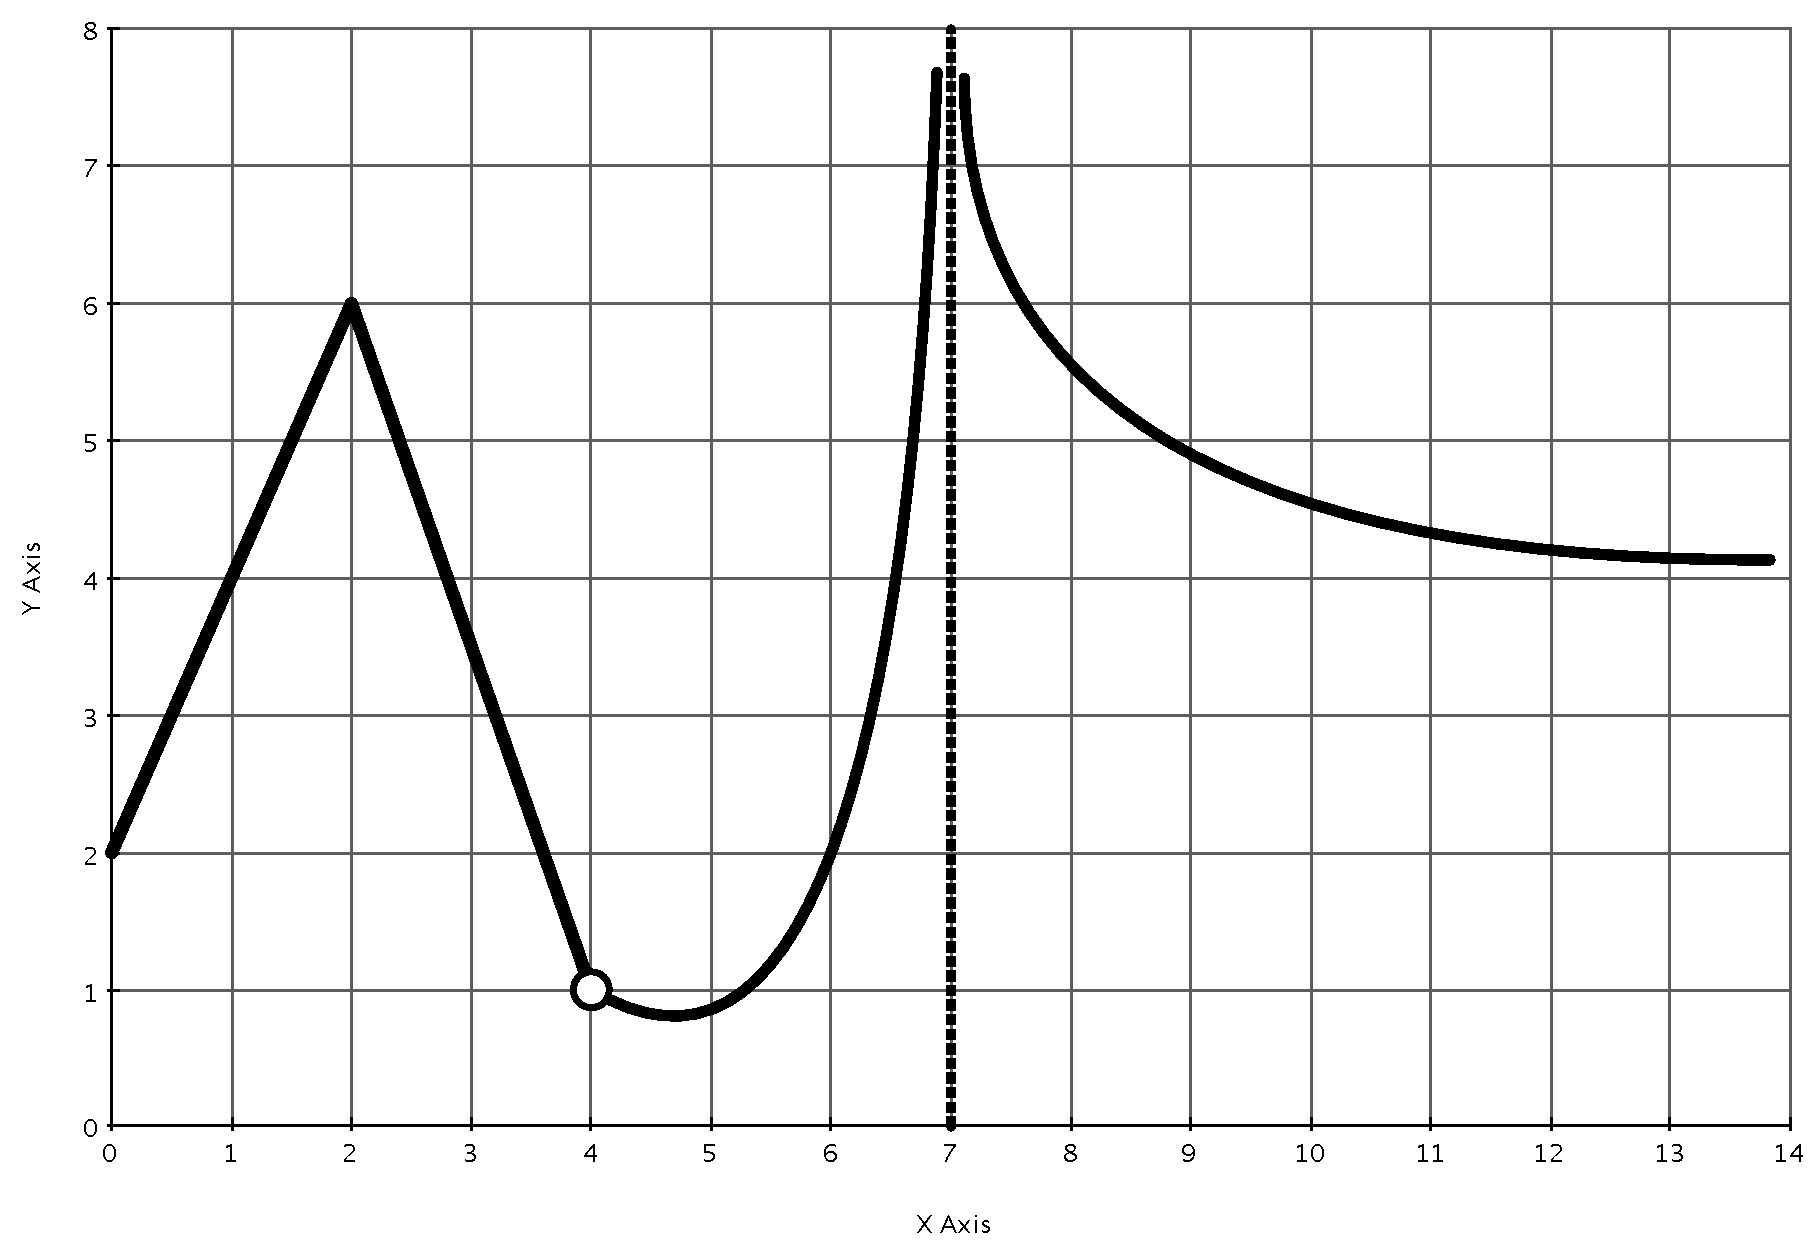
\includegraphics[width=0.5\textwidth]{fe-graphlimits}
\end{center}
	\begin{parts}
		\part[2] State the value of $\displaystyle{\lim_{x \to 4} f(x)}$. If the limit fails to exist, say so. 
		\vspace{0.75in}
		
		\part[2] State the value of $\displaystyle{\lim_{x \to \infty} f(x)}$. If the limit fails to exist, say so. 
		\vspace{0.75in}
		
		\part[2] State the $x$-values of the points where $f$ is discontinuous. 
		\vspace{0.75in}
		
		
		\part[2] State the $x$-values of the points where $f$ fails to be differentiable. 
		\vspace{0.75in}

		
		\part[4] Estimate the instantaneous rate of change in $f$ at $x = 6$. 
		
	\end{parts}

\pageturn

\question Consider the function $f(x) = 2x^2 - 5x + 10$. 
	\begin{parts}
		\part[4] Use the definition of the derivative to set up an expression involving limits that would calculate the value of $f'(2)$. 
		
		\vspace{1.5in}
		
		\part[8] Evaluate the limit expression you set up in the previous part to find $f'(2)$. Show all work. Work that does not involve evaluating a limit will receive no credit.
		
		\vspace{3.5in}
		
		\part[4] Find the equation of the tangent line to the graph of $f$ at $x = 2$. 
	\end{parts}
	
\pageturn

\question Compute each of the following derivatives using the computational rules developed in Chapter 2 of our book. That is, DO NOT use the limit definition of the derivative. Show all work and fully simplify all results. 
	\begin{parts}
		\part[8] $y = (2 + 9x^2)^{3/2}$
		
		\vspace{2.5in}
		
		\part[8] $y = \dfrac{8}{1 + \cot x}$
		
		\vspace{2.5in}
		
		\part[8] $y = \ln(\arcsin (x))$ 
	\end{parts}




\pageturn 


\question Bob walks into his kitchen and turns on the hot water to wash off a pan. The  temperature of the water ($T$, in degrees Fahrenheit) after $t$ seconds of the water running is given in the following table: 
\begin{center}
	\begin{tabular}{c||c|c|c|c|c|c}
	$t$ (seconds) & 0 & 2 & 4 & 6 & 8 & 10 \\ \hline
	$T$ (degrees F) & 60 & 79.8 & 93.0 & 101.9 & 107.9 & 111.9 
	\end{tabular}
\end{center}

\begin{parts}
	\part[6] How fast is the temperature climbing after 8 seconds? Give the best estimate you can using only the data in the table; show all work and put correct units on the answer. 
	
	\vspace{2in}
	
	\part[8] Find the linearization of $T$ at $t = 8$, and use the linearization to predict the water's temperature after 15 seconds.
	
	\vspace{2in}
	 

	
	\part[8] A model for the temperature function is $T(t) = 120 - 60e^{-0.2t}$. Using derivative rules, find the exact value of the instantaneous rate of change in the temperature at $t=8$. (Note that you estimated this value in part (a), so both answers should be relatively close to each other in value.) 
	
\end{parts}


%\pageturn

%\question Given graph of $f'$, state behaviors 

\pageturn

\question[16] Choose EXACTLY ONE of the following problems to solve, and then solve it by giving a complete, clear, and correct solution that is supported by mathematical calculations. You will lose credit for solutions that are unclear, messy, or consist ONLY of calculations with no explanatory text. Clearly indicate which problem you are doing by circling the bullet point next to it. Providing significant work on more than one problem will result in a grade of ``0'' on this problem. 
	\begin{itemize}
		\item A rectangular storage container with an open top is to have a
		volume of 10 \(m^3\). The length of its base is twice the
		width. Material for the base costs \$15 per \(m^2\). Material
		for the sides costs \$16 per \(m^2\). Find the dimensions of
		the container which will minimize cost and the minimum cost.
		\item A water filter is in the shape of an inverted right circular cone with a height of 8cm and radius 6 cm. If water drips out of the cone so that the water level inside the cone is dropping at a constant rate of 0.1cm per minute, find the rate in which the radius of the surface of the water is changing at the instant the height of the water level is 4cm. 
	\end{itemize}




\pageturn

\question Below is the graph of a function $f(x)$. The two parts of the graph are semicircles. 
\begin{center}
	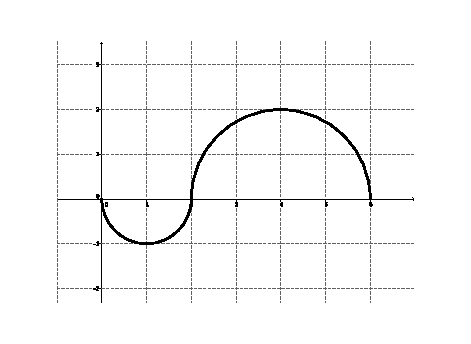
\includegraphics[width=0.5\textwidth]{fe-integration}
\end{center}

	\begin{parts}
		\part[6] Estimate the value of $\int_0^6 f(x) \, dx$ using the Riemann sum $M_3$. 
		
		\vspace{1in}
		
		\part[6] Compute the exact value of the integral. Do not use any decimal approximations and show all work. 
		
		\vspace{1in}
		
	\end{parts}

\question For each of the integrals below, use an antiderivative to find the exact value of the integral, using no decimal approximations. 
	\begin{parts}
		% \part[8] $\displaystyle{\int_0^1 (4x^3 - 2x^5) \, dx}$ 
		% 
		% \vspace{1in}
		
		\part[8] $\displaystyle{\int_1^2 \frac{x^3 + 1}{x} \, dx}$
		
		\vspace{1.5in}
		
		\part[8] $\displaystyle{\int_0^{\pi/4} \sec^2 x \, dx}$
	\end{parts}

\pageturn

\question The graph below shows the rate ($r$, in hundreds of people per hour) at which people enter and leave a basketball game as a function of time ($t$, in hours since 2:00pm) from 2:00pm to 5:00pm. (That is, from $t=0$ to $t=3$.) 
\begin{center}
	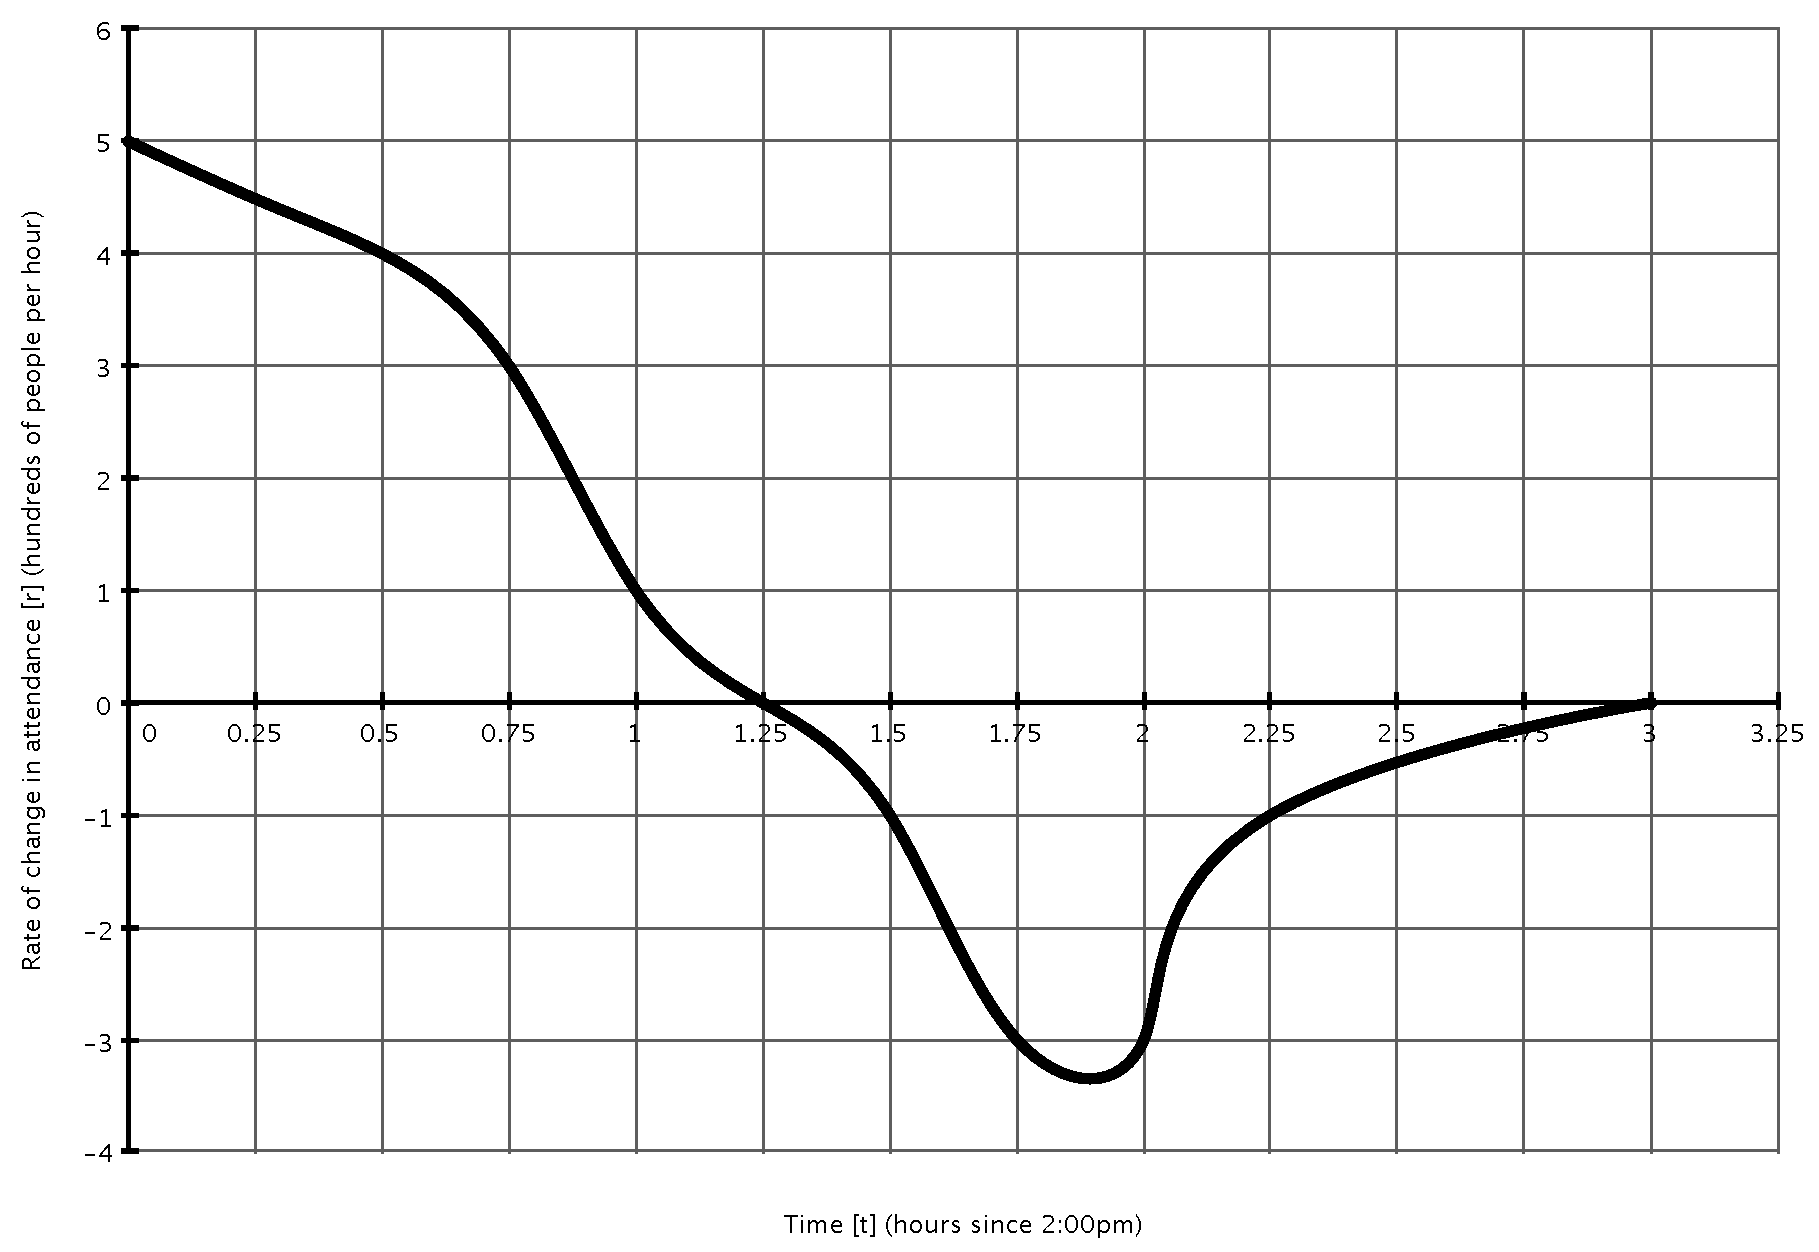
\includegraphics[width=0.5\textwidth]{fe-totalchange}
\end{center}

\begin{parts}
	\part[6] At what time was the attendance at the basketball game greatest? State your answer and then explain how you know. 
	\vspace{2in}
	
	\part[6] Estimate the total net change in the attendance at the basketball game from 2:00pm to 5:00pm. Show all your work and explain how you got your estimate. 
	

\end{parts}


\end{questions}


\end{document}